\chapter{THIẾT KẾ CƠ SỞ DỮ LIỆU QUAN HỆ CHUẨN 3NF}

\section{Mô hình thực thể liên kết (Entity Relationship Diagram - ERD)}

Cơ sở dữ liệu của hệ thống được thiết kế theo đúng các chuẩn mực thiết kế CSDL quan hệ, đạt chuẩn hóa dạng 3NF (Third Normal Form). Mọi bảng dữ liệu đều có khóa chính đơn nhất, các thuộc tính phi khóa đều phụ thuộc trực tiếp vào khóa chính và không có phụ thuộc bắc cầu.

Toàn bộ lược đồ CSDL gồm 11 bảng quan hệ liên kết chặt chẽ qua các khóa ngoại với ràng buộc toàn vẹn tham chiếu nghiêm ngặt:

\begin{figure}[h!]
\centering
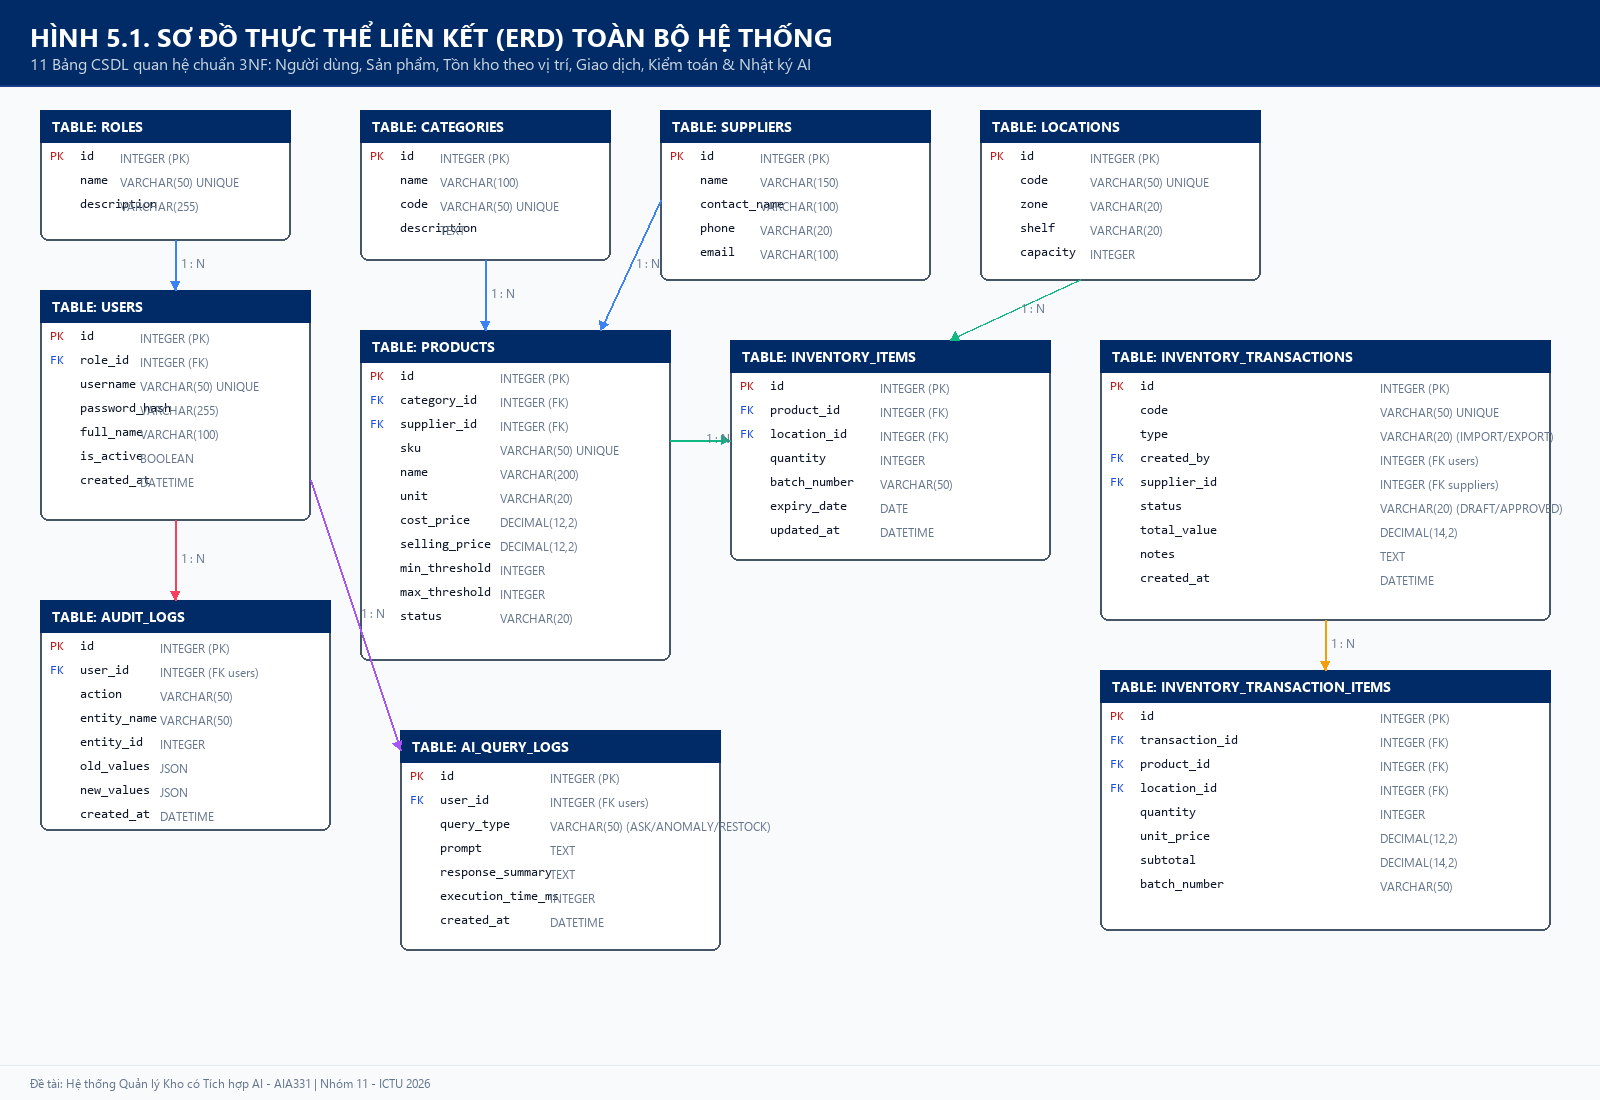
\includegraphics[width=0.92\textwidth]{figures/erd.png}
\caption{Sơ đồ thực thể liên kết (ERD) 11 bảng chuẩn 3NF của hệ thống quản lý kho}
\end{figure}

\section{Đặc tả chi tiết các bảng dữ liệu trong hệ thống}

Dưới đây là đặc tả chi tiết cấu trúc, kiểu dữ liệu, khóa chính, khóa ngoại và ràng buộc của 11 bảng trong cơ sở dữ liệu:

\begin{table}[h!]
\centering
\caption{Đặc tả cấu trúc bảng người dùng (users)}
\begin{tabular}{|l|l|l|l|l|}
\hline
\rowcolor{tablehead}
\textbf{Tên cột} & \textbf{Kiểu dữ liệu} & \textbf{Khóa} & \textbf{Ràng buộc} & \textbf{Mô tả nghiệp vụ} \\ \hline
id & INTEGER & PK & AUTO\_INCREMENT & Mã định danh duy nhất của người dùng \\ \hline
username & VARCHAR(50) & None & UNIQUE, NOT NULL & Tên đăng nhập hệ thống \\ \hline
email & VARCHAR(100) & None & UNIQUE, NOT NULL & Địa chỉ email của nhân sự \\ \hline
hashed\_password & VARCHAR(255) & None & NOT NULL & Mật khẩu đã được băm bằng Argon2 \\ \hline
full\_name & VARCHAR(100) & None & NOT NULL & Họ và tên đầy đủ của nhân sự \\ \hline
role & VARCHAR(20) & None & NOT NULL & Vai trò: ADMIN, WAREHOUSE, ACCOUNTANT \\ \hline
is\_active & BOOLEAN & None & DEFAULT TRUE & Trạng thái kích hoạt tài khoản \\ \hline
created\_at & DATETIME & None & DEFAULT UTC\_NOW & Thời điểm tạo tài khoản \\ \hline
\end{tabular}
\end{table}

\begin{table}[h!]
\centering
\caption{Đặc tả cấu trúc bảng nhóm sản phẩm (categories)}
\begin{tabular}{|l|l|l|l|l|}
\hline
\rowcolor{tablehead}
\textbf{Tên cột} & \textbf{Kiểu dữ liệu} & \textbf{Khóa} & \textbf{Ràng buộc} & \textbf{Mô tả nghiệp vụ} \\ \hline
id & INTEGER & PK & AUTO\_INCREMENT & Mã nhóm sản phẩm \\ \hline
name & VARCHAR(100) & None & NOT NULL & Tên nhóm (Linh kiện, Màn hình, Phụ kiện) \\ \hline
code & VARCHAR(20) & None & UNIQUE, NOT NULL & Mã định danh nhóm hàng \\ \hline
description & TEXT & None & NULL & Mô tả chi tiết nhóm hàng \\ \hline
created\_at & DATETIME & None & DEFAULT UTC\_NOW & Thời điểm tạo nhóm \\ \hline
\end{tabular}
\end{table}

\begin{table}[h!]
\centering
\caption{Đặc tả cấu trúc bảng đơn vị tính (units)}
\begin{tabular}{|l|l|l|l|l|}
\hline
\rowcolor{tablehead}
\textbf{Tên cột} & \textbf{Kiểu dữ liệu} & \textbf{Khóa} & \textbf{Ràng buộc} & \textbf{Mô tả nghiệp vụ} \\ \hline
id & INTEGER & PK & AUTO\_INCREMENT & Mã đơn vị tính \\ \hline
name & VARCHAR(50) & None & NOT NULL & Tên đơn vị (Chiếc, Hộp, Bộ, Thùng) \\ \hline
code & VARCHAR(20) & None & UNIQUE, NOT NULL & Mã ký hiệu đơn vị \\ \hline
description & TEXT & None & NULL & Mô tả chi tiết \\ \hline
\end{tabular}
\end{table}

\begin{table}[h!]
\centering
\caption{Đặc tả cấu trúc bảng nhà cung cấp (suppliers)}
\begin{tabular}{|l|l|l|l|l|}
\hline
\rowcolor{tablehead}
\textbf{Tên cột} & \textbf{Kiểu dữ liệu} & \textbf{Khóa} & \textbf{Ràng buộc} & \textbf{Mô tả nghiệp vụ} \\ \hline
id & INTEGER & PK & AUTO\_INCREMENT & Mã nhà cung cấp \\ \hline
code & VARCHAR(20) & None & UNIQUE, NOT NULL & Mã định danh đối tác cung cấp \\ \hline
name & VARCHAR(150) & None & NOT NULL & Tên công ty / đơn vị phân phối \\ \hline
contact\_person & VARCHAR(100) & None & NULL & Người liên hệ trực tiếp \\ \hline
phone & VARCHAR(20) & None & NULL & Số điện thoại liên lạc \\ \hline
email & VARCHAR(100) & None & NULL & Thư điện tử liên hệ \\ \hline
address & TEXT & None & NULL & Địa chỉ trụ sở đối tác \\ \hline
is\_active & BOOLEAN & None & DEFAULT TRUE & Trạng thái hợp tác \\ \hline
created\_at & DATETIME & None & DEFAULT UTC\_NOW & Thời điểm tạo đối tác \\ \hline
\end{tabular}
\end{table}

\begin{table}[h!]
\centering
\caption{Đặc tả cấu trúc bảng sản phẩm (products)}
\begin{tabular}{|l|l|l|l|l|}
\hline
\rowcolor{tablehead}
\textbf{Tên cột} & \textbf{Kiểu dữ liệu} & \textbf{Khóa} & \textbf{Ràng buộc} & \textbf{Mô tả nghiệp vụ} \\ \hline
id & INTEGER & PK & AUTO\_INCREMENT & Mã định danh sản phẩm \\ \hline
code & VARCHAR(50) & None & UNIQUE, NOT NULL & Mã SKU quản lý kho \\ \hline
name & VARCHAR(200) & None & NOT NULL & Tên quy chuẩn của sản phẩm \\ \hline
category\_id & INTEGER & FK & REFERENCES categories(id) & Khóa ngoại trỏ về nhóm hàng \\ \hline
unit\_id & INTEGER & FK & REFERENCES units(id) & Khóa ngoại trỏ về đơn vị tính \\ \hline
cost\_price & NUMERIC(15,2) & None & NOT NULL, >= 0 & Giá vốn nhập kho quy chuẩn \\ \hline
selling\_price & NUMERIC(15,2) & None & NOT NULL, >= 0 & Giá niêm yết bán ra \\ \hline
minimum\_stock & INTEGER & None & DEFAULT 0, >= 0 & Định mức tồn an toàn tối thiểu \\ \hline
maximum\_stock & INTEGER & None & DEFAULT 0, >= 0 & Định mức tồn kho tối đa \\ \hline
location & VARCHAR(50) & None & NULL & Ký hiệu vị trí kệ lưu trữ \\ \hline
is\_active & BOOLEAN & None & DEFAULT TRUE & Trạng thái kinh doanh \\ \hline
created\_at & DATETIME & None & DEFAULT UTC\_NOW & Thời điểm tạo sản phẩm \\ \hline
\end{tabular}
\end{table}

\begin{table}[h!]
\centering
\caption{Đặc tả cấu trúc bảng tồn kho hiện tại (inventory)}
\begin{tabular}{|l|l|l|l|l|}
\hline
\rowcolor{tablehead}
\textbf{Tên cột} & \textbf{Kiểu dữ liệu} & \textbf{Khóa} & \textbf{Ràng buộc} & \textbf{Mô tả nghiệp vụ} \\ \hline
id & INTEGER & PK & AUTO\_INCREMENT & Mã định danh bản ghi tồn \\ \hline
product\_id & INTEGER & FK & UNIQUE, REFERENCES products(id) & Khóa ngoại 1-1 trỏ về sản phẩm \\ \hline
quantity & INTEGER & None & NOT NULL, DEFAULT 0, >= 0 & Số lượng hàng thực tế trong kho \\ \hline
updated\_at & DATETIME & None & DEFAULT UTC\_NOW & Thời điểm cập nhật biến động gần nhất \\ \hline
\end{tabular}
\end{table}

\begin{table}[h!]
\centering
\caption{Đặc tả cấu trúc bảng phiếu nhập kho (import_receipts)}
\begin{tabular}{|l|l|l|l|l|}
\hline
\rowcolor{tablehead}
\textbf{Tên cột} & \textbf{Kiểu dữ liệu} & \textbf{Khóa} & \textbf{Ràng buộc} & \textbf{Mô tả nghiệp vụ} \\ \hline
id & INTEGER & PK & AUTO\_INCREMENT & Mã phiếu nhập \\ \hline
code & VARCHAR(50) & None & UNIQUE, NOT NULL & Số hiệu chứng từ nhập kho \\ \hline
supplier\_id & INTEGER & FK & REFERENCES suppliers(id) & Nhà cung cấp giao hàng \\ \hline
user\_id & INTEGER & FK & REFERENCES users(id) & Nhân viên lập phiếu nhập \\ \hline
receipt\_date & DATETIME & None & NOT NULL & Thời điểm giao nhận hàng hóa \\ \hline
total\_amount & NUMERIC(15,2) & None & DEFAULT 0.0 & Tổng giá trị tiền hàng nhập \\ \hline
status & VARCHAR(20) & None & DEFAULT 'COMPLETED' & Trạng thái phiếu nhập \\ \hline
note & TEXT & None & NULL & Ghi chú giao nhận \\ \hline
created\_at & DATETIME & None & DEFAULT UTC\_NOW & Thời điểm tạo phiếu trên hệ thống \\ \hline
\end{tabular}
\end{table}

\begin{table}[h!]
\centering
\caption{Đặc tả cấu trúc bảng chi tiết phiếu nhập kho (import_receipt_details)}
\begin{tabular}{|l|l|l|l|l|}
\hline
\rowcolor{tablehead}
\textbf{Tên cột} & \textbf{Kiểu dữ liệu} & \textbf{Khóa} & \textbf{Ràng buộc} & \textbf{Mô tả nghiệp vụ} \\ \hline
id & INTEGER & PK & AUTO\_INCREMENT & Mã dòng chi tiết nhập \\ \hline
receipt\_id & INTEGER & FK & REFERENCES import\_receipts(id) & Thuộc về phiếu nhập nào \\ \hline
product\_id & INTEGER & FK & REFERENCES products(id) & Sản phẩm được nhập \\ \hline
quantity & INTEGER & None & NOT NULL, > 0 & Số lượng nhập thực tế \\ \hline
unit\_price & NUMERIC(15,2) & None & NOT NULL, >= 0 & Đơn giá nhập của từng sản phẩm \\ \hline
total\_price & NUMERIC(15,2) & None & NOT NULL, >= 0 & Thành tiền (quantity * unit\_price) \\ \hline
\end{tabular}
\end{table}

\begin{table}[h!]
\centering
\caption{Đặc tả cấu trúc bảng phiếu xuất kho (export_receipts)}
\begin{tabular}{|l|l|l|l|l|}
\hline
\rowcolor{tablehead}
\textbf{Tên cột} & \textbf{Kiểu dữ liệu} & \textbf{Khóa} & \textbf{Ràng buộc} & \textbf{Mô tả nghiệp vụ} \\ \hline
id & INTEGER & PK & AUTO\_INCREMENT & Mã phiếu xuất kho \\ \hline
code & VARCHAR(50) & None & UNIQUE, NOT NULL & Số hiệu chứng từ xuất kho \\ \hline
user\_id & INTEGER & FK & REFERENCES users(id) & Thủ kho lập phiếu xuất \\ \hline
receipt\_date & DATETIME & None & NOT NULL & Thời điểm xuất kho thực tế \\ \hline
receiver & VARCHAR(150) & None & NOT NULL & Đơn vị hoặc người nhận hàng \\ \hline
total\_amount & NUMERIC(15,2) & None & DEFAULT 0.0 & Tổng giá trị tiền hàng xuất \\ \hline
status & VARCHAR(20) & None & DEFAULT 'COMPLETED' & Trạng thái phiếu xuất \\ \hline
note & TEXT & None & NULL & Lý do và ghi chú xuất hàng \\ \hline
created\_at & DATETIME & None & DEFAULT UTC\_NOW & Thời điểm tạo phiếu trên hệ thống \\ \hline
\end{tabular}
\end{table}

\begin{table}[h!]
\centering
\caption{Đặc tả cấu trúc bảng chi tiết phiếu xuất kho (export_receipt_details)}
\begin{tabular}{|l|l|l|l|l|}
\hline
\rowcolor{tablehead}
\textbf{Tên cột} & \textbf{Kiểu dữ liệu} & \textbf{Khóa} & \textbf{Ràng buộc} & \textbf{Mô tả nghiệp vụ} \\ \hline
id & INTEGER & PK & AUTO\_INCREMENT & Mã dòng chi tiết xuất \\ \hline
receipt\_id & INTEGER & FK & REFERENCES export\_receipts(id) & Thuộc về phiếu xuất nào \\ \hline
product\_id & INTEGER & FK & REFERENCES products(id) & Mặt hàng được xuất \\ \hline
quantity & INTEGER & None & NOT NULL, > 0 & Số lượng xuất kho \\ \hline
unit\_price & NUMERIC(15,2) & None & NOT NULL, >= 0 & Đơn giá xuất \\ \hline
total\_price & NUMERIC(15,2) & None & NOT NULL, >= 0 & Thành tiền của dòng xuất \\ \hline
\end{tabular}
\end{table}

\begin{table}[h!]
\centering
\caption{Đặc tả cấu trúc bảng nhật ký biến động kho (stock_movements)}
\begin{tabular}{|l|l|l|l|l|}
\hline
\rowcolor{tablehead}
\textbf{Tên cột} & \textbf{Kiểu dữ liệu} & \textbf{Khóa} & \textbf{Ràng buộc} & \textbf{Mô tả nghiệp vụ} \\ \hline
id & INTEGER & PK & AUTO\_INCREMENT & Mã nhật ký biến động \\ \hline
product\_id & INTEGER & FK & REFERENCES products(id) & Mặt hàng phát sinh biến động \\ \hline
movement\_type & VARCHAR(20) & None & NOT NULL & Loại biến động: IMPORT, EXPORT, ADJUST \\ \hline
quantity & INTEGER & None & NOT NULL & Số lượng biến động (+ tăng, - giảm) \\ \hline
previous\_stock & INTEGER & None & NOT NULL & Số lượng tồn trước biến động \\ \hline
new\_stock & INTEGER & None & NOT NULL & Số lượng tồn sau biến động \\ \hline
reference\_id & INTEGER & None & NULL & Mã chứng từ liên kết (receipt id) \\ \hline
reference\_type & VARCHAR(50) & None & NULL & Loại chứng từ tham chiếu \\ \hline
user\_id & INTEGER & FK & REFERENCES users(id) & Nhân sự thực hiện thao tác \\ \hline
note & TEXT & None & NULL & Diễn giải chi tiết lý do biến động \\ \hline
created\_at & DATETIME & None & DEFAULT UTC\_NOW & Dấu thời gian phát sinh giao dịch \\ \hline
\end{tabular}
\end{table}

\section{Ràng buộc toàn vẹn dữ liệu, chỉ mục (Indexing) và tối ưu hóa}

Hệ thống áp dụng các quy tắc ràng buộc toàn vẹn cấp CSDL nghiêm ngặt:

1. Ràng buộc khóa chính và khóa ngoại có kiểm tra toàn vẹn tham chiếu (FOREIGN KEY ... REFERENCES). Khi xóa một danh mục hoặc sản phẩm, hệ thống ngăn chặn hành vi xóa nếu đã phát sinh phiếu xuất nhập liên kết (RESTRICT).

2. Ràng buộc giá trị không âm: Sử dụng CHECK constraint cho các trường số lượng và đơn giá (quantity >= 0, unit\_price >= 0), bảo đảm không có giá trị bất thường đi vào CSDL.

3. Tối ưu hóa truy vấn bằng chỉ mục (Indexes): Đánh chỉ mục B-Tree trên các trường thường xuyên tìm kiếm và nối bảng: products(code), products(category\_id), stock\_movements(product\_id, created\_at), import\_receipts(receipt\_date), export\_receipts(receipt\_date). Việc này giúp giảm thời gian truy vấn báo cáo từ O(N) xuống O(log N).

